%!TEX root = ..\..\main.tex
\chapter{Maximum Likelihood Location Mixtures}
\label{Ch:Mixtures}

\lhead{Chapter \ref{Ch:Mixtures}. \emph{Maximum Likelihood Location Mixtures}}

\graphicspath{{Figures/Mixtures/}}

%-------------------------------------------------------------------------------
%	Chapter Text
%-------------------------------------------------------------------------------

\section{Introduction}
	Mixtures of distributions have been used to model a wide variety of phenomena, with successful applications in the fields of ``astronomy, biology, genetics, medicine, psychiatry, economics, engineering, and marketing, among many other fields in the biological, physical, and social sciences'' \cite[Section 1.1.1]{McLachlan2004-ik}. Mixture models have been in use for over 100 years. In 1984, Pearson used a mixture of two normal densities to model the distribution of the ratio of forehead to body lengths of a sample of 1000 crabs \cite{Pearson1894-qv}. His mixture of two normals was able to account for the skewness in the data, which a single normal could not model. Pearson suggested that this signalled the existence of two sub-populations of crabs; each associated with its own normal distribution.

	However, we do not require that data comes from a mixture of distributions in any physical sense for mixtures to be a useful modelling tool. 
	One of the traits that has contributed to the extent of the use of mixtures is that they provide a convenient semi-parametric way of modelling unknown distributions. They are particularly useful in situations where a parametric method is too restrictive to satisfactorily model the data, and a fully non-parametric method, such as kernel density estimation, may require evaluating a sum which contains more terms than desired. By way of illustration, Priebe in \cite{Priebe1994-ng} discussed modelling a log normal density using a mixture of normals. With $n = 10000$ observations, Priebe only required about 30 normals to obtain a good approximation. This is in contrast to a kernel density estimator which in this case would be essentially a mixture of 10000 normals.

	% [WHAT ELSE?]

	% \subsection{Definitions}
	A \emph{mixture density} is a probability density function that can be written in the form
	\begin{equation}
		f_Q(\vect{x}) = \int_\Omega f(\vect{x}; \vect{\theta}) \intd Q(\vect{\theta})
		\label{eq:mixture definition}
	\end{equation}
	where $f(\vect{x};\vect{\theta})$ is the \emph{component density}, parametrised by $\vect{\theta} \in \Omega$, and $Q$ is a probability distribution on $\Omega$, called the \emph{mixing distribution}. In the case that $Q$ is a discrete probability distribution, with probability masses $p_j$ at points $\vect{\theta}_j$, $j = 1, \dots, m$, the mixture density in \eqref{eq:mixture definition} is a \emph{finite mixture} and can be written
	\begin{equation}
		f_Q(\vect{x}) = f_{\vect{\theta}, \vect{p}}(\vect{x}) = \sum_{j = 1}^m p_j f(\vect{x}; \vect{\theta}_j).
	\end{equation}

	In this chapter, we will be concerned only with finite mixtures on the real line, whose component densities are parametrised by a single shifting parameter, $\theta$. This is what we will call a \emph{location mixture}, and it can be written as
	\begin{equation}
		f_{\vect{p}, \vect{\theta}} = \sum_{j = 1}^m p_j f(x - \theta_j)
		\label{eq:location mixture}
	\end{equation}
	for a single component density $f(x)$.
	Looking only at mixtures of this form is not as restrictive as it may at first seem. Using a finite location mixture of normals, you can approximate any continuous density arbitrarily well [BETTER CITATION] \cite{McLachlan2004-ik}.

	A common question when using mixtures is the following. Let $\vect{X} = (X_1, \dots, X_n)$ be a random sample of size $n$, where $X_i$ has probability density function $g(\vect{x})$. Given $\vect{x} = (x_1, \dots, x_n)$, an observed random sample of $\vect{X}$, and a component density $f(\vect{x}; \vect{\theta})$, how do we choose the mixing distribution $Q$ so that $f_Q(\vect{x})$ is a good approximation for $g(\vect{x})$?	One answer to this question is to choose $Q$ to maximise the likelihood.

	The \emph{likelihood} of a distribution $Q$ given $\vect{x}$ is 
	\begin{equation}
		L(Q;\vect{x}, f) = \prod_{i = 1}^n f_Q(x_i).
	\end{equation}
	Maximizing $L(Q;\vect{x}, f)$ may be achieved by instead maximizing the \emph{log likelihood},
	\begin{equation}
		l(Q; \vect{x}, f) = \log L(Q; \vect{x}, f) = \sum_{i = 1}^n \log f_Q(x_i),
		\label{eq:loglikelihood}
	\end{equation}
	since $\log(x)$ is a strictly increasing function. In \cite{Lindsay1983-tf}, Lindsay showed that so long as the likelihood is bounded, there exists a maximizing $Q$ that has at most $n$ points of support. This is a useful result because it means that the problem of finding a maximizing $Q$ is an optimization problem having finite dimensions. It also justifies our decision to only consider finite mixtures in this chapter.

	% While one can construct examples in which the mixing distribution that maximizes the likelihood has all $n$ points of support, in practise, 
	The size of the support of the $Q$ that maximizes \eqref{eq:loglikelihood} is the primary quantity of interest for this Chapter. We define it as follows. Let $\mathcal{Q}_n$ be the set of all discrete probability distributions on $\mathbb{R}$ with no more than $n$ points of support. Let
	\begin{equation}
		\hat{Q}_{\vect{x},f} = \{Q \in \mathcal{Q}_n: \forall Q' \in \mathcal{Q}_n, l(Q;\vect{x}) \geq l(Q';\vect{x})\}
	\end{equation}
	be the set of all global maximizers of \eqref{eq:loglikelihood}. Then define
	\begin{equation}
		K_\vect{x} = K(\vect{x}; f) = \min\{m \leq n : \mathcal{Q}_m \cap \hat{Q}_{\vect{x},f} \neq \emptyset\}
	\end{equation}
	which counts the smallest number of probability masses needed to maximize the likelihood.


	There are a few considerations to be made here. The first is that there is not necessarily a unique mixing distribution that maximizes \eqref{eq:loglikelihood} and so we have defined the quantity of interest as the smallest number of points of support required for a maximizing distribution. However, in many cases, including most cases where the component density is from the exponential family, we know that the maximizing mixing distribution is unique. This question of uniqueness was addressed by Lindsay in \cite{Lindsay1983-tf} and in \cite{Lindsay1983a-he} for univariate component densities in the exponential family. A generalization of these results can be found in \cite{Lindsay1993-rj}.

	The second, is that our choice to only consider location mixtures is significant in that it guarantees the likelihood to be bounded so long as the component density is bounded. In general, this is not the case. Consider the likelihood function for a mixture of normals parametrized by both the mean and variance. We can create a mixture by placing equally weighted normals with very small variance at each $x_i$ in our sample. This corresponds to a mixing distribution $Q$ which places probability mass $1/n$ at points $(x_i, \sigma^2)$ for $i = 1, \dots, n$. As $\sigma^2$ approaches zero, the density at each $x_i$, $f_Q(x_i)$, increases without bound and so the likelihood is unbounded. There are a number of techniques that can be employed to ensure the likelihood is bounded such as restricting the parameter space appropriately or restricting the number of components to some number that grows slowly with $n$ (the sieve method \cite{Grenander1981-dy}).

	The third, is that we should be careful to make a distinction between calculating $K_\vect{x}$ and choosing an appropriate number of components for a mixture model. The former is simply a deterministic property of an optimization problem whereas the latter is an in-depth and difficult problem which involves consideration of properties such as consistency, and the use of techniques such as information criteria and likelihood ratio. This latter problem is discussed in \cite[Chapter 6]{McLachlan2004-ik}. In particular, if each $X_i$ comes from a distribution with density $g(x) = f_Q(x)$ (that is, $g(x)$ is a mixture density itself) then we may consider the `true' number of components and using certain penalised log likelihood criteria, such as the Akaike information criterion (AIC) \cite{Akaike1974-bl} or the Bayesian information criterion (BIC) \cite{Schwarz1978-ci}, does not underestimate this quantity asymptotically \cite{Leroux1992-ek}. This suggests that we should not expect $K_\vect{x}$ (which is defined from an unpenalised likelihood) to necessarily be reflective of the properties of $g(x)$.
 
	% Not necessarily unique Q
	% Location mixtures only (otherwise unbounded likelihood and use all n points)
	% Mention sieves
	% NOT about recovering the 'true' number of components - we are using mixtures as a density approximation tool and are interested in the property of this optimization.

	% A location mixture on $\mathbb{R}$ with mixing distribution $Q$ and component density $f(x)$ can be written as
	% \begin{equation}
	% 	f_Q(x) = \int_{-\infty}^\infty f(x-\theta) \intd Q(\theta).
	% \label{eq:mixtureint}
	% \end{equation}

	% Given a sample $\vect{x} = (x_1,\dots,x_n)$, we wish to find a distribution that maximizes the log likelihood	
	% \begin{equation}
	% 	L(Q;\vect{x}) = \sum_{i = 1}^n \log(f_Q(x_i)).
	% \label{eq:loglikelihood}
	% \end{equation}
	% Lindsay showed that under quite general conditions, such a maximizing distribution exists and has no more than $n$ points of support \cite{Lindsay1983-tf}. It is therefore common to use
	% \begin{equation}
	% 	f_{\vect{p},\vect{\theta}}(x) = \sum_{j = 1}^m p_j f(x - \theta_j)
	% \label{eq:mixturesum}
	% \end{equation}
	% instead of \eqref{eq:mixtureint} as our definition of a location mixture. We note that \eqref{eq:mixtureint} is equivalent to \eqref{eq:mixturesum} in the case where $Q$ is a discrete distribution which places probability masses of weight $p_j$ at locations $\theta_j$, for $j = 1,\dots,m$. The order of the $x_i$ does not matter and so we will assume without loss of generality that $x_1 \leq x_2 \leq \dots \leq x_n$ throughout.
	
	% In this paper we are primarily interested in the number of probability masses that are required in the maximizing mixture. We will call this quantity $K_{\vect{x}}$. It should be noted that there is not always a unique mixing distribution that maximizes \eqref{eq:loglikelihood}. However we can choose $K_{\vect{x}}$ to be the smallest number of probability masses that any of the maximizing distributions have.
\section{Summary of Lindsay}
	To obtain results concerning $K_\vect{x}$ we will make use of the geometrical approach employed by Lindsay in \cite{Lindsay1983-tf} and \cite{Lindsay1983a-he} and summarized later in \cite[Chapter 5]{Lindsay1995-sq}. This section is dedicated to laying out the basics of this approach and summarising the results that are most relevant to our work. Here, we assume that the component densities, $f(\vect{x};\vect{\theta})$, are bounded, but we do not restrict ourselves to finite location mixtures on the real line.

	\subsection{The likelihood curve}
	The key to Lindsay's approach is to reformulate the problem from optimizing over all mixing distributions, to optimizing an appropriate objective function over a convex set in $\mathbb{R}^n$. Define the \emph{likelihood vector}
	\begin{equation}
		\vect{\gamma}(Q;\vect{x}, f) = (f_Q(x_1), \dots, f_Q(x_n))
		\label{eq:likelihood vector}
	\end{equation}
	and the objective function
	\begin{equation}
		\mathcal{L}(\vect{\gamma}) = \sum_{i = 1}^n \ln(\gamma_i).
	\end{equation}
	Let 
	\begin{equation}
		\mathcal{M} = \{\vect{\gamma}(Q;\vect{x}, f): \text{$Q$ is a probability distribution}\}
	\end{equation}
	be the set of all possible values of the likelihood vector. A maximizing mixing distribution may be found by first finding the $\hat{\vect{\gamma}} \in \mathcal{M}$ that maximizes $\mathcal{L}(\vect{\gamma})$ and then solving the $n$ equations
	\begin{equation}
		\vect{\gamma}(Q; \vect{x}, f) = \hat{\vect{\gamma}}
	\end{equation}
	for $Q$.

	To show that $\mathcal{M}$ is a convex set, consider the \emph{unicomponent likelihood vector}
	\begin{equation}
		\vect{\gamma}(\vect{\theta}; \vect{x}, f) = (f_\vect{\theta}(x_1), \dots, f_\vect{\theta}(x_n))
	\end{equation}
	where $f_\vect{\theta}$ is the mixture density corresponding to the mixing distribution that places all its mass at $\vect{\theta}$, that is, 
	\begin{equation}
		f_\vect{\theta}(x) = f(x; \vect{\theta}).
	\end{equation}
	For any probability distribution, $Q$, the likelihood vector can be represented by
	\begin{equation}
		\vect{\gamma}(Q; \vect{x}, f) = \int \vect{\gamma}(\vect{\theta}; \vect{x}, f) \intd Q(\vect{\theta})
	\end{equation}
	which for a finite mixture $Q$, with weights $p_j$ assigned to parameters $\vect{\theta}_j$, can be written as
	\begin{equation}
		\vect{\gamma}(Q;\vect{x},f) = \sum_{j = 1}^m p_j \vect{\gamma}(\vect{\theta}_j; \vect{x}, f).
	\end{equation}
	
	This leads to an alternative characterisation of $\mathcal{M}$. Define the \emph{unicomponent likelihood curve}
	\begin{equation}
		\Gamma_{\vect{x}, f} = \{\vect{\gamma}(\vect{\theta}; \vect{x}, f) : \vect{\theta} \in \Omega\}.
	\end{equation}
	Then
	\begin{equation}
		\mathcal{M} = \conv(\Gamma_{\vect{x}, f}),
	\end{equation}
	where we use $\conv(A)$ to denote the convex hull of $A$. We now state the following Theorem taken directly from \cite[Theorem 18]{Lindsay1995-sq} which is a consequence of the convexity of $\mathcal{M}$, and the concavity of $\mathcal{L}(\vect{\gamma})$.

	\begin{theorem}[\cite{Lindsay1995-sq}]
		Suppose that $\Gamma_{\vect{x}, f}$ is closed and bounded and that $\mathcal{M}$ contains at least one point with positive likelihood. Then there exists a unique $\hat{\vect{\gamma}} \in \partial \mathcal{M}$, the boundary of $\mathcal{M}$, such that $\hat{\vect{\gamma}}$ maximizes $\mathcal{L}(\vect{\gamma})$ over $\mathcal{M}$.
		\label{thm: lindsay maximizing likelihood vector point}
	\end{theorem}

	In addition to this, in \cite[Theorem 21]{Lindsay1995-sq} is stated the following.
	\begin{theorem}[\cite{Lindsay1995-sq}]
		The solution $\hat{\vect{\gamma}}$ can be represented as $\vect{\gamma}(\hat{Q};\vect{x}, f)$, where $\hat{Q}$ has no more than $n$ points of support.
		\label{thm: lindsay no more than n points}
	\end{theorem}
	This gives us our first bound on $K_\vect{x}$: for component densities that produce a closed and bounded likelihood curve,
	\begin{equation}
		K_\vect{x} \leq n.
	\end{equation}

	% \subsection{The likelihood curve}
	% 	In \cite{Lindsay1983-tf}, the problem of mixture likelihoods was looked at from a geometrical perspective. One key construction introduced by Lindsay was the \emph{likelihood curve},
	% 	\begin{equation}
	% 		\vect{\gamma}(\theta;\vect{x}) = (f(x_{1}-\theta),\dots,f(x_{n}-\theta))
	% 		\label{eq:Gamma}
	% 	\end{equation}
	% 	and it's trace,
	% 	\begin{equation}
	% 		\Gamma_{\vect{x}} = \{\vect{\gamma}(\theta;\vect{x})| \theta \in \mathbb{R}\}.
	% 	\end{equation}
	% 	A useful property of the likelihood curve is that any convex combination of elements from $\Gamma_{\vect{x}}$ can be written as
	% 	\begin{equation}
	% 		\vect{u}(\vect{p},\vect{\theta};\vect{x}) = (f_{\vect{p},\vect{\theta}}(x_{1}),\dots,f_{\vect{p},\vect{\theta}}(x_{n})) = \sum_{j = 1}^m p_j \vect{\gamma}(\theta_j;\vect{x}), \hspace{30pt} \sum_{j=1}^m p_j = 1
	% 		\label{eq:convexcombinationgamma}
	% 	\end{equation}
	% 	where $f_{\vect{p},\vect{\theta}}(x)$ is as defined in \eqref{eq:mixturesum}. The log likelihood of the corresponding distribution is simply the sum of the log of the components of $\vect{u}(\vect{p},\vect{\theta};\vect{x})$.
		
	% 	One of Lindsay's main results, which follows from this observation, was that if
	% 	\begin{equation}
	% 		\hat{\vect{u}} = \argmax_{\vect{u} \in \conv(\Gamma_{\vect{x}})} \sum_{i=1}^n \log(u_i)
	% 		\label{eq:optimalu}
	% 	\end{equation}
	% 	% where
	% 	% \begin{equation}
	% 	% 	U =  %\{\vect{u}(\vect{p},\vect{\theta};\vect{x}) |  \}
	% 	% \end{equation}
	% 	then we can write
	% 	\begin{equation}
	% 		\hat{\vect{u}} = \vect{u}(\vect{p},\vect{\theta};\vect{x})
	% 	\end{equation}
	% 	for some $\vect{p}$ and $\vect{\theta}$ whose dimension is no more than $n$. Furthermore, the corresponding distribution that places masses $p_j$ at locations $\theta_j$ maximizes \eqref{eq:loglikelihood}. There are some minor conditions on this result, but they will not cause any problems for our purposes and so will not be discussed (see \cite{Lindsay1983-tf} for details).
	\subsection{An example likelihood curve}
		\label{sec:mixturelikelihoods:example}
		In simple cases, we can plot the likelihood curve, $\Gamma_{\vect{x}, f}$, and objective function, $\mathcal{L}$, along with the maximizing point, $\hat{\vect{\gamma}}$. In particular, when $n = 2$, $\Gamma_{\vect{x}, f} \subset \mathbb{R}^2$ and if the component density is smoothly parametrized by a single parameter, then we can plot $\Gamma_{\vect{x}, f}$ by tracing out $\vect{\gamma}(\theta; \vect{x}, f)$ as we vary $\theta$.

		For example, suppose our sample is made up of two points, $\vect{x} = (x_1, x_2) = (1,2)$, and suppose our component density is normal with variance $\sigma_2 = 0.45^2$ and parametrized by $\theta$, that is,
		\begin{equation}
		f(x;\theta) = \frac{1}{0.45 \sqrt{2 \pi}} \exp\left(-\frac{(x-\theta)^2}{2\cdot 0.45^2}\right).
		\label{eq:example component density for likelihood curve}
		\end{equation}
		Then the corresponding likelihood curve can be traced out as we increase $\theta$ from $-\infty$ to $\infty$ as shown in Figure \ref{fig:TracingGamma}. 

		\begin{figure}[ht]
			\centering
			\begin{minipage}[b]{0.3\linewidth}
				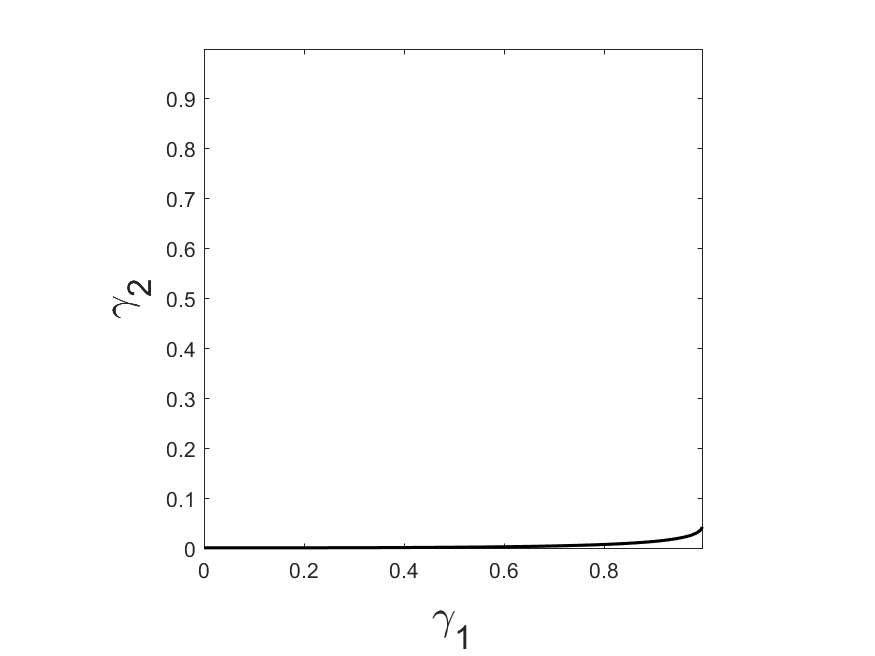
\includegraphics[width=\textwidth]{GammaTrace01}
			\end{minipage}
			\begin{minipage}[b]{0.3\linewidth}
				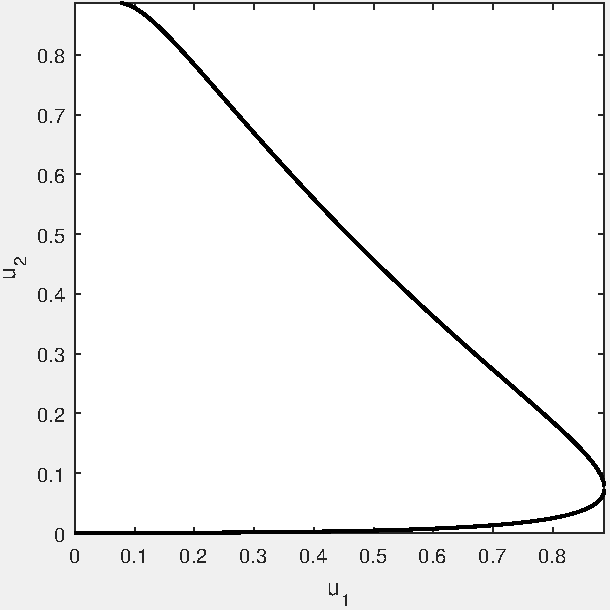
\includegraphics[width=\textwidth]{GammaTrace02}
			\end{minipage}
			\begin{minipage}[b]{0.3\linewidth}
				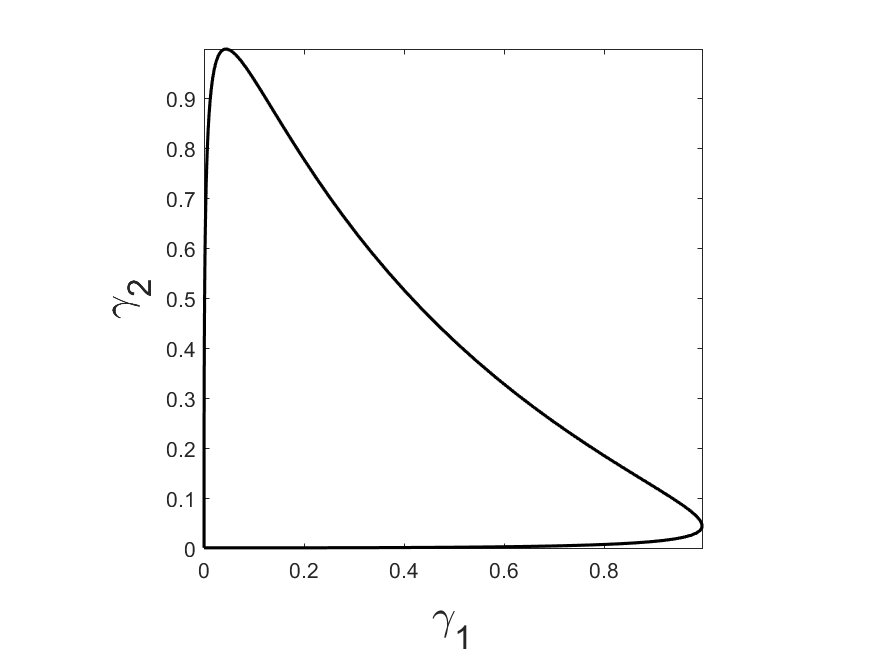
\includegraphics[width=\textwidth]{GammaTrace03}
			\end{minipage}
			\begin{minipage}[b]{0.3\linewidth}
				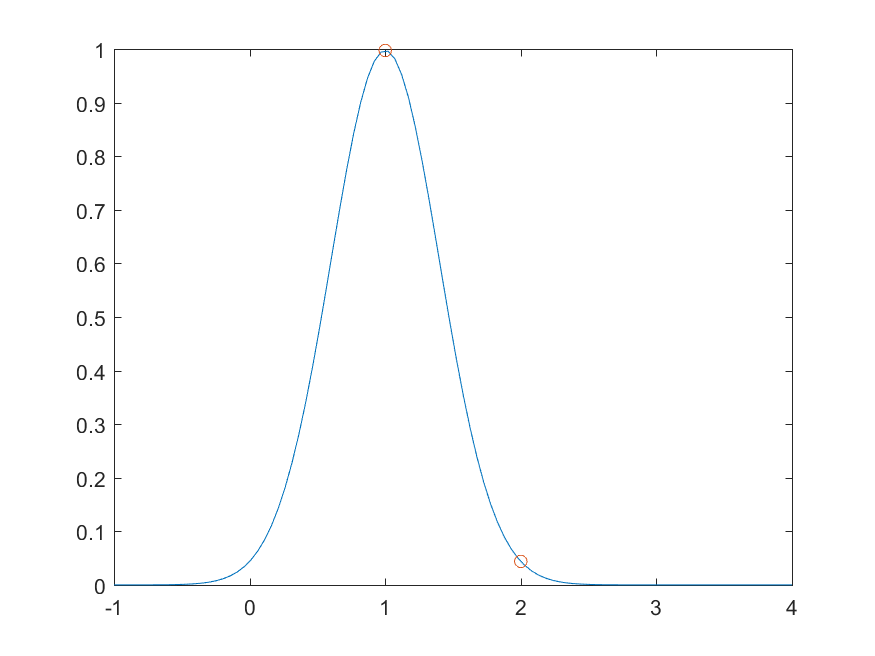
\includegraphics[width=\textwidth]{GammaTraceDensity01}
				\subcaption{$\theta = 1$}
			\end{minipage}
			\begin{minipage}[b]{0.3\linewidth}
				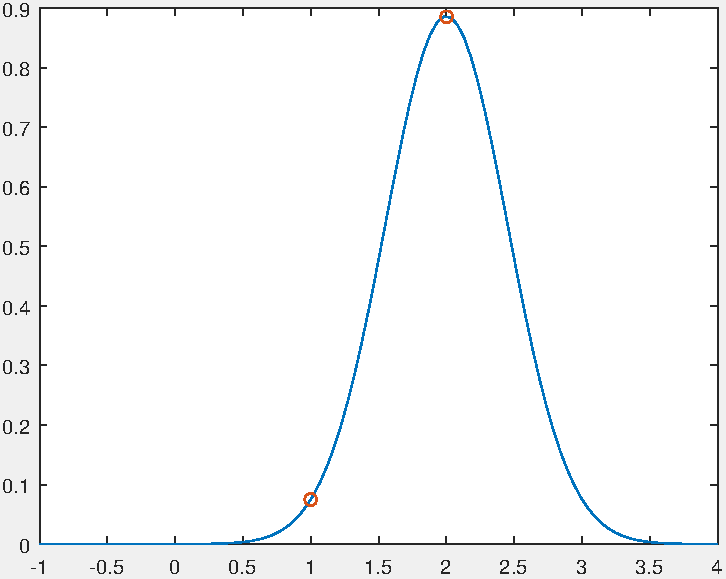
\includegraphics[width=\textwidth]{GammaTraceDensity02}
				\subcaption{$\theta = 2$}
			\end{minipage}
			\begin{minipage}[b]{0.3\linewidth}
				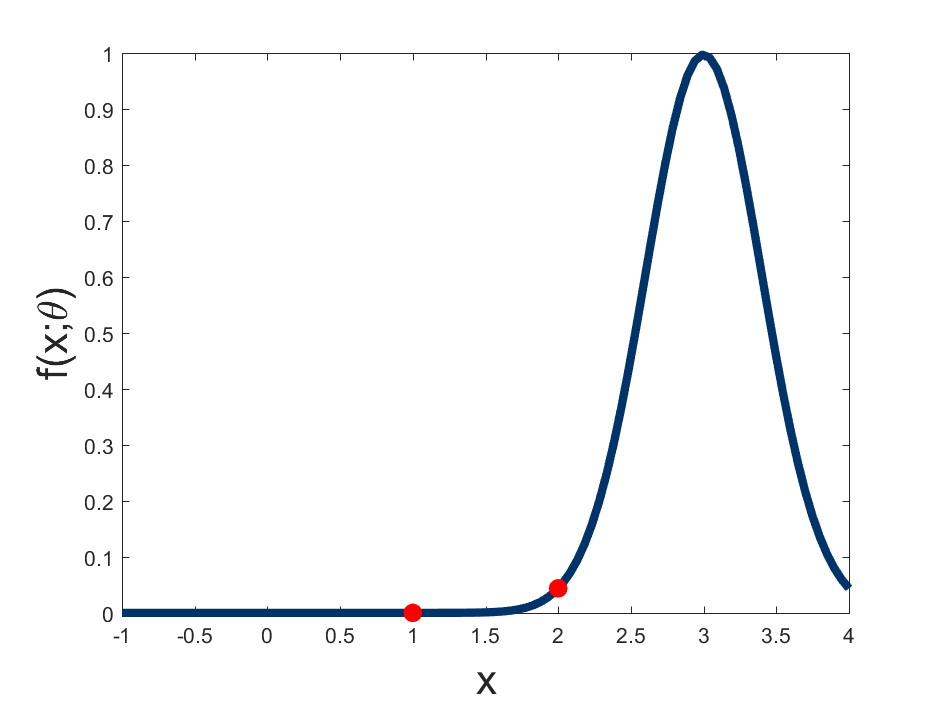
\includegraphics[width=\textwidth]{GammaTraceDensity03}
				\subcaption{$\theta = 3$}
			\end{minipage}
			\caption[A simple example of a likelihood curve.]{A simple example of a likelihood curve. The component density, $f(x;\theta)$, as defined in \eqref{eq:example component density for likelihood curve}, is shown in blue for $\theta = 1,2,$ and $3$. Each value of $\theta$ contributes a point to $\Gamma_{\vect{x}, f}$ whose coordinates are given by $(f(1;\theta),f(2;\theta))$ (represented by the red circles). As we increase $\theta$ from $-\infty$ to $\infty$ we trace out more of $\Gamma_{\vect{x}, f}$.}\label{fig:TracingGamma}
		\end{figure}

		[MAKE THIS FIGURE REPRODUCIBLE?]
		
		The set of possible values of the likelihood vector, $\mathcal{M}$, is given by the convex hull of $\Gamma_{\vect{x}, f}$, the boundary of which is marked along with $\Gamma_{\vect{x}, f}$ in Figure \ref{fig:GammaSol:subfig:Gamma} and overlaid on a heat map of $\mathcal{L}(\vect{\gamma})$. The maximizing point, $\hat{\vect{\gamma}}$, is marked with a yellow dot and lies on the boundary of $\conv(\Gamma_{\vect{x}, f})$ as predicted by Theorem \ref{thm: lindsay maximizing likelihood vector point}. This point may be written as the convex combination of two points in $\Gamma_{\vect{x}, f}$,
		\begin{equation}
			\hat{\vect{\gamma}} = \sum_{j = 1}^2 p_j \vect{\gamma}(\theta_j;\vect{x}, f)
		\end{equation}
		and we represent the two points, $\vect{\gamma}(\theta_1;\vect{x}, f)$ and $\vect{\gamma}(\theta_2;\vect{x}, f)$ with magenta dots.

		The mixture $\hat{Q}$ that satisfies $\hat{\vect{\gamma}} = \vect{\gamma}(\hat{Q};\vect{x}, f)$ is the one that places masses $p_1$ and $p_2$ at locations $\theta_1$ and $\theta_2$ and it is plotted in Figure \ref{fig:GammaSol:subfig:Density} by two magenta points at $(\theta_1, p_1)$ and $(\theta_2, p_2)$ along with the overall mixture density $f_{\hat{Q}}(x)$.

		% The optimal point is on the boundary of $\conv(\Gamma)$ as expected and it can be written as the  $p_1 \vect{f}(\theta_1) + p_2 \vect{f}(\theta_2)$ (where $p_1 + p_2 =1 $). These two points correspond to the two probability masses in the maximizing mixture distribution shown in Figure \ref{fig:GammaSol:subfig:Density}. These masses are located at $\theta_1$ and $\theta_2$ with weights $p_1$ and $p_2$.

		%and so we will provide a slightly more general form of Theorem \ref{thm:LindsayGamma}.
		%\begin{theorem}
		%	Write $\vect{0}$ for the zero vector in $\mathbb{R}^n$. If $\Gamma \cup \{ \vect{0} \}$ is compact then there exists a unique point on the boundary of $\conv(\Gamma)$ which maximizes the likelihood. This point corresponds to a distribution $Q$ which maximizes the likelihood and that has no more than $n$ point masses.
		%\end{theorem}
		%\begin{proof}
		%	We need to show that $\vect{0}$ does not appear in the maximizing mixture. Clearly, $\vect{0}$ is not going to be a maximizing point.
		%\end{proof}

		% We trace the boundary of $\conv(\Gamma)$ in Figure \ref{fig:GammaSol} along with a heat map of the objective function \eqref{eq:transformedlikelihood}.

		\begin{figure}[ht]
			\centering
			\begin{minipage}{0.4\textwidth}
				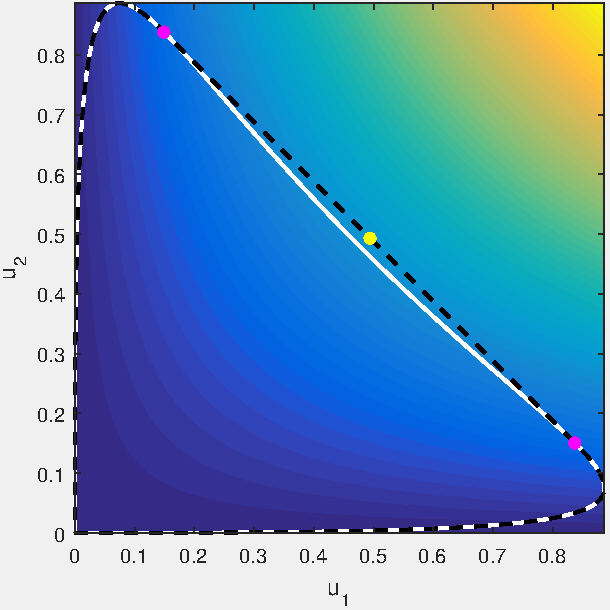
\includegraphics[width = \textwidth]{GammaOptimHullSol}
				\subcaption{}\label{fig:GammaSol:subfig:Gamma}
			\end{minipage}
			\begin{minipage}{0.5\textwidth}
				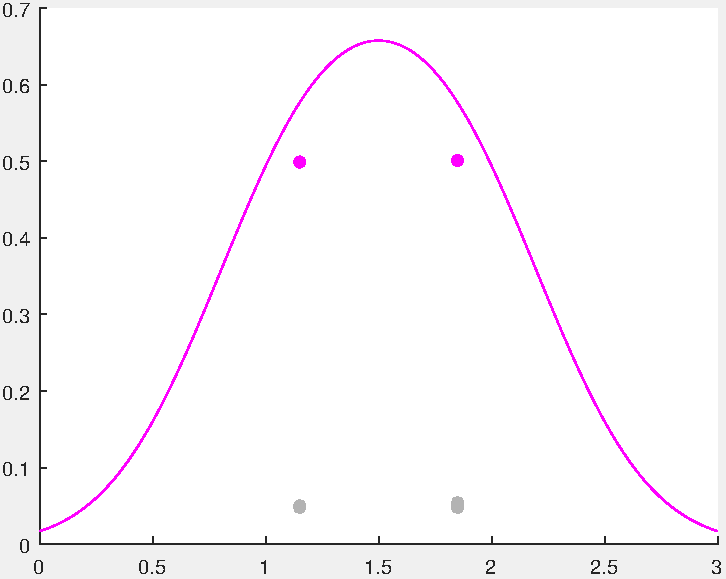
\includegraphics[width = \textwidth]{MixingSolSigma045}				\subcaption{}\label{fig:GammaSol:subfig:Density}
			\end{minipage}
			\caption[The geometric relationship between the likelihood curve (\subref{fig:GammaSol:subfig:Gamma}) and the maximizing mixture density (\subref{fig:GammaSol:subfig:Density}).]{The geometric relationship between the likelihood curve (\subref{fig:GammaSol:subfig:Gamma}) and the maximizing mixture density (\subref{fig:GammaSol:subfig:Density}). In (\subref{fig:GammaSol:subfig:Gamma}), the boundary of $\conv(\Gamma_{\vect{x}, f})$ is shown as a dashed black line, $\Gamma_{\vect{x}, f}$ is the white curve, the heat map  shows the objective function (likelihood increases from blue to yellow) and $\hat{\vect{\gamma}}$ is marked with a yellow dot. This point is a convex combination of the two magenta points. These two magenta points correspond to the two probability masses in the maximizing mixing distribution (\subref{fig:GammaSol:subfig:Density}).}
			\label{fig:GammaSol}
		\end{figure}

		[MAKE THIS FIGURE REPRODUCIBLE + FIX]

		\begin{remark}
			Note that in this example, while $\Gamma_{\vect{x}, f}$ is bounded, it is not closed (it does not contain the limit point $(0,0)$), counter to the requirements of Theorems \ref{thm: lindsay maximizing likelihood vector point} and \ref{thm: lindsay no more than n points}. In fact, any positive density whose support is the whole real line will not contain the limit point $\vect{0}$ (where $\vect{0}$ represents the zero vector in $\mathbb{R}^n$). However, since $\vect{0}$ is clearly not going to be a part of a maximizing mixture, we are safe to apply both theorems if $\Gamma \cup \{ \vect{0} \}$ is closed. A more detailed discussion concerning how to relax the requirement that the set $\Gamma_{\vect{x},f}$ be closed can be found in \cite[Section 5.2.2.]{Lindsay1995-sq}.
		\end{remark}

	\subsection{Gradient characterization}
	Another important construction due to Lindsay is the gradient function
	\begin{equation}
		D_Q(\vect{\theta}; \vect{x}, f) = -n + \sum_{i = 1}^n \frac{f(x_i;\vect{\theta})}{f_Q(x_i)}.
	\end{equation}
	This is the derivative of $l(Q;\vect{x},f)$ as we move along the path parametrized by
	\begin{equation}
		(1 - p)Q + p\Delta_\vect{\theta}
	\end{equation}
	evaluated at $p = 0$ and where $\Delta_\vect{\theta}$ is a degenerate distribution that places all of its mass at $\vect{\theta}$. In \cite[Theorem 4.1]{Lindsay1983-tf}, Lindsay showed you could characterise the maximizing mixture by three equivalent conditions. The statement of the Theorem here is taken from \cite[Theorem 19]{Lindsay1995-sq}.

	\begin{theorem}[\cite{Lindsay1995-sq}]
	\label{thm:Lindsay three statements that characterise maximizing mixture}
		The following three statements are equivalent:
		\begin{enumerate}
			\item $\hat{Q}$ maximizes $l(Q;\vect{x},f)$.
			\item $\hat{Q}$ minimizes $\sup_\vect{\theta} D_Q(\vect{\theta};\vect{x}, f)$.
			\item $\sup_\vect{\theta} D_{\hat{Q}}(\vect{\theta};\vect{x}, f) = 0$.
			\label{item:supremum of gradient is zero}
		\end{enumerate}
	\end{theorem}

	Also contained in \cite[Theorem 4.1]{Lindsay1983-tf} was the following result concerning the locations of the support points of $\hat{Q}$. The statement here is taken from \cite[Theorem 20]{Lindsay1995-sq}.

	\begin{theorem}[\cite{Lindsay1995-sq}]
		\label{thm: Lindsay support is zeros of gradient}
		The support of any maximum likelihood estimator $\hat{Q}$ lies in the set 
		\begin{equation}
			\left\{\vect{\theta} : D_{\hat{Q}}(\vect{\theta};\vect{x},f) = 0 \right\}.
		\end{equation}
	\end{theorem}

	If $f$ is parametrized by a single parameter $\theta$ and $D_Q(\theta;\vect{x},f)$ is twice differentiable in $\theta$, then each interior support point $\theta^*$ of the maximizing mixture distribution, $\hat{Q}$, satisfies
	\begin{align}
		D_{\hat{Q}}(\theta^*;\vect{x}, f) &= 0, 
		\label{eq:Deq1}\\
		D'_{\hat{Q}}(\theta^*;\vect{x}, f) &= 0, 
		\label{eq:Deq2}\\
		D''_{\hat{Q}}(\theta^*;\vect{x}, f) &\leq 0.
		\label{eq:Deq3}
	\end{align}

	\subsubsection{Support Hyperplane}
	There is a geometrical interpretation to these theorems that ties in with the likelihood curve interpretation given above. For any given mixing distribution $Q$, define the \emph{inverse likelihood vector} $\vect{\gamma}^{-1}(Q;\vect{x},f) = (1/f_Q(x_1),\dots, 1/f_Q(x_n))$ and the hyperplane
	\begin{equation}
		\mathcal{H}_{Q} = \{\vect{z} : \langle \vect{\gamma}^{-1}(Q;\vect{x},f), \vect{z}\rangle = n\},
	\end{equation}
	which contains the usual likelihood vector, $\vect{\gamma}(Q;\vect{x}, f)$. We may write the gradient function as
	\begin{equation}
		D(Q;\vect{x},f) = \langle \vect{\gamma}^{-1}(Q;\vect{x},f), \vect{\gamma}(\vect{\theta};\vect{x},f)\rangle - n.
	\end{equation}
	If $\hat{Q}$ maximizes $l(Q;\vect{x},f)$ then by statement \ref{item:supremum of gradient is zero}, 
	\begin{equation}
		\langle \vect{\gamma}^{-1}(\hat{Q};\vect{x},f), \vect{\gamma}(\vect{\theta};\vect{x},f) \rangle \leq n
	\end{equation}
	for all $\vect{\theta} \in \Omega$. This means that $\mathcal{M} = \conv(\Gamma_{\vect{x},f})$ lies entirely on one side of $\mathcal{H}$ and Theorem \ref{thm: Lindsay support is zeros of gradient} tell us that if $\vect{\theta}$ is in the support of $\hat{Q}$, then 
	\begin{equation}
		\langle \vect{\gamma}^{-1}(\hat{Q};\vect{x},f), \vect{\gamma}(\vect{\theta};\vect{x},f) \rangle = n
	\end{equation}
	and so $\vect{\gamma}(\vect{\theta};\vect{x},f) \in \mathcal{H}$. Thus the question of determining the number of support points of $\hat{Q}$ can be answered by finding the number of points at which $\Gamma_{\vect{x},f}$ touches $\mathcal{H}_{\hat{Q}}$.

	[FIGURE]

	\subsection{Additional results on \texorpdfstring{$K_\vect{x}$}{Kx}}

	Theorem \ref{thm: lindsay no more than n points} bounds $K_\vect{x}$ by $n$. To get tighter bounds on $K_\vect{x}$, we must make some assumptions about the form of the component densities, or the structure of $\vect{x}$.

	[FOLLOWING IS NOTES FOR MYSELF]

	Exponential family \cite{Lindsay1983a-he}, more general results including this one and others in \cite{Lindsay1993-rj}. In particular, $n/2$ for discrete densities. May want to cite \cite{Seregin2010-xe} since it has some very limited results on the support. Read \cite{Zhang2008-wn} for more citations.
	

	% \subsection{Directional Derivative}
	% 	One of the tools introduced in \cite{Lindsay1983-tf} was the function
	% 	\begin{equation}
	% 		D(\theta;\vect{p},\vect{\theta},\vect{x}) = -n + \sum_{i=1}^n \frac{f(x_i - \theta)}{\sum_{j=1}^m p_j f(x_i - \theta_j)}.
	% 	\end{equation}

	% 	Lindsay showed that if $\hat{\vect{\theta}}$ and $\hat{\vect{p}}$ form a maximum likelihood location mixture of $f$ for $\vect{x}$ then (under appropriate differentiability assumuptions) the function $D$ satisfies the following:
	% 	% \begin{align}
	% 	% 	D(\theta_k;\hat{\vect{p}},\hat{\vect{\theta}},\vect{x}) &= 0, && k = 1,\dots,m,
	% 	% 	\label{eq:Deq1}\\
	% 	% 	D'(\theta_k;\hat{\vect{p}},\hat{\vect{\theta}},\vect{x}) &= 0, && k = 1,\dots,m,
	% 	% 	\label{eq:Deq2}\\
	% 	% 	D''(\theta_k;\hat{\vect{p}},\hat{\vect{\theta}},\vect{x}) &\leq 0, && k = 1,\dots,m.
	% 	% 	\label{eq:Deq3}
	% 	% \end{align}
	% 	These three constraints restrict what a potential maximum likelihood solution can look like.
	% 	HOW DID LINDSAY USE THEM VS US?


\section{Numerical Results}
	In this section we explore $K_\vect{x}$ through empirical results and figures. The process we use to generate the results is essentially the same throughout. We choose $\vect{x} \in \mathbb{R}^n$ either deterministically or randomly, and use a general purpose nonlinear programming solver to find the maximum likelihood mixture (we use the MATLAB function \emph{fmincon}). We can test that we have indeed reached the global maximum through the use of the derivative function conditions given in Theorem \ref{thm:Lindsay three statements that characterise maximizing mixture}. If the mixture that is returned by our general solver does not satisfy these conditions then we may use another method, such as the vertex direction method (VDM) or the vertex exchange method (VEM), which is guaranteed to converge to the global maximum (see \cite{Bohning1995-di} for a review of different methods). We note that the actual method used is not important so long as the final result satisfies the derivative conditions. In practise, we deal with $\vect{x} \in \mathbb{R}^n$ with $n$ small, for which a general purpose solver is sufficient, fast, and simple to implement, and we rarely need to use a secondary method.

	[MAY WISH TO BE MORE SPECIFIC HERE BUT WILL NEED TO REWRITE CODE TO MATCH]

	We initiate our general purpose solver with a mixture distribution that has more points of support than is needed. Under the optimization, this collapses down to a distribution which may assign zero weight to some masses, and may concentrate multiple masses on the one point of support (see Figure [MAKE FIGURE]). We may simplify such a distribution by removing all masses with zero weight, and by combining all masses which share a point of support into one mass which takes the combined weight of the constituent masses. The number of probability masses in this simplified distribution is the value we take for $K_\vect{x}$.

	Throughout this section, and for the remainder of this chapter, we will consider only location mixtures (see \eqref{eq:location mixture}). All component densities will be unimodal, with a mode at $x = 0$. We list here the component densities that we will use.

	\begin{tabular}{l | c}
		Density & $f(x) = $\\
		\hline
		normal with fixed variance $\sigma^2$ & $\frac{1}{\sigma \sqrt{2 \pi}} \exp\left(-\frac{x^2}{2\sigma^2}\right) $\\
		Cauchy with fixed scale $\gamma$ & $\frac{1}{\pi \gamma + \pi x^2/\gamma}$
	\end{tabular}

	[EXTEND AS REQUIRED]
	% \subsection{Motivating Example?}

	\subsection{Flag graphs}
	When is $n$ is very small, we can plot $K_\vect{x}$ as a function of $\vect{x}$. For example, we may take $\vect{x} = (x_1, x_2)$ across a grid of values and colour each point $\vect{x}$ according to the value of $K_\vect{x}$. We have done this in Figure \ref{fig:normal_flag_graph_n2} for a normal component density with fixed variance $\sigma^2 = 1$. We observe a band in which $K_\vect{x} = 1$ and outside of which $K_\vect{x} = 2$.

	\begin{figure}
		\centering
		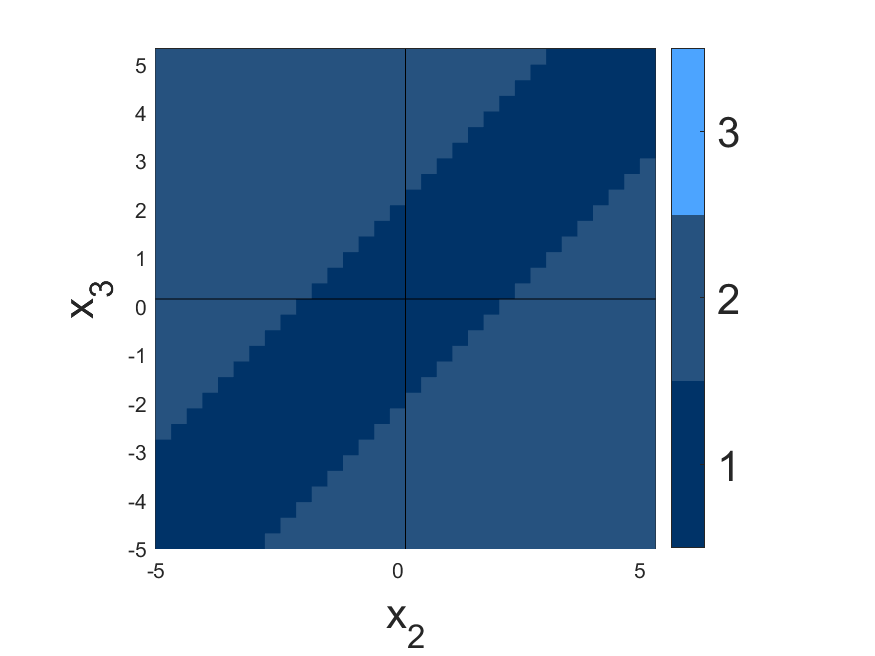
\includegraphics[width = 0.9\textwidth]{Figures/Mixtures/normal_flag_graph_n2.png}
		\caption{$K_\vect{x}$ as a function of $\vect{x} = (x_1, x_2)$, for a normal component density with fixed variance $\sigma^2 = 1$.}
		\label{fig:normal_flag_graph_n2}
	\end{figure}

	However, there is some redundancy in this plot which arises because we are using location mixtures. When using a location mixture, if the maximizing mixing distribution for $\vect{x}$ places weights $p_j$ at locations $\theta_j$, then a maximizing mixing distribution for $\vect{x} + (c, \dots, c)$ for some constant $c \in \mathbb{R}$ is simply the distribution that places weights $p_j$ at locations $\theta_j + c$. That is, shifting $\vect{x}$ by $c$ results in the maximizing mixture also shifting by $c$. A consequence of this fact is that $K_\vect{x}$ is invariant under translations of $\vect{x}$.

	This suggests increases $n$ to $3$, and fixing one of the $x_i$ while letting the other two vary. We do this by taking $\vect{x} = (0, x_2, x_3)$ with $x_2$ and $x_3$ varying across an evenly spaced grid. We do this for both a normal component density with variance $\sigma^2 = 1$ (Figure \ref{fig:normal_flag_graph}) and a Cauchy density with scale $\gamma = \sqrt{3}$ (Figure \ref{fig:cauchy_flag_graph}). We have chosen the scale of the Cauchy so that it has inflection points in the same places as the normal density, namely at $x = \pm 1$. This decision is made in light of Theorem \ref{thm:n=2 inflection result} which says that for $n = 2$ and for certain component densities $f$, $K_\vect{x}$ can be determined by comparing $|x_1 - x_2|$ and the distance between the inflection points of $f$. It seems reasonable to expect that the choice of scale that makes the $n = 2$ figures identical is a good choice for comparing the effects of choosing different component densities in the $n = 3$ case.

	% One point that we wish to emphasize is that, given a component density $f$, $K$ is a function of $\vect{x}$ only. We can visualise this for small values of $n$. In Figure \ref{fig:normal_flag_graph}, we empirically found the MLE for $\vect{x} = (0,x_2,x_3)$ and recorded the number of probability masses in the maximizing mixture. We took values for $x_2$ and $x_3$ from an evenly spaced grid with $-6\leq x_2,x_3\leq 6$. We fixed $x_1 = 0$ since the shape of the maximum likelihood mixture (and therefore $K_{\vect{x}}$) depends only on the relative location of the $x_i$, not their absolute location.
	
	\begin{figure}
		\centering
		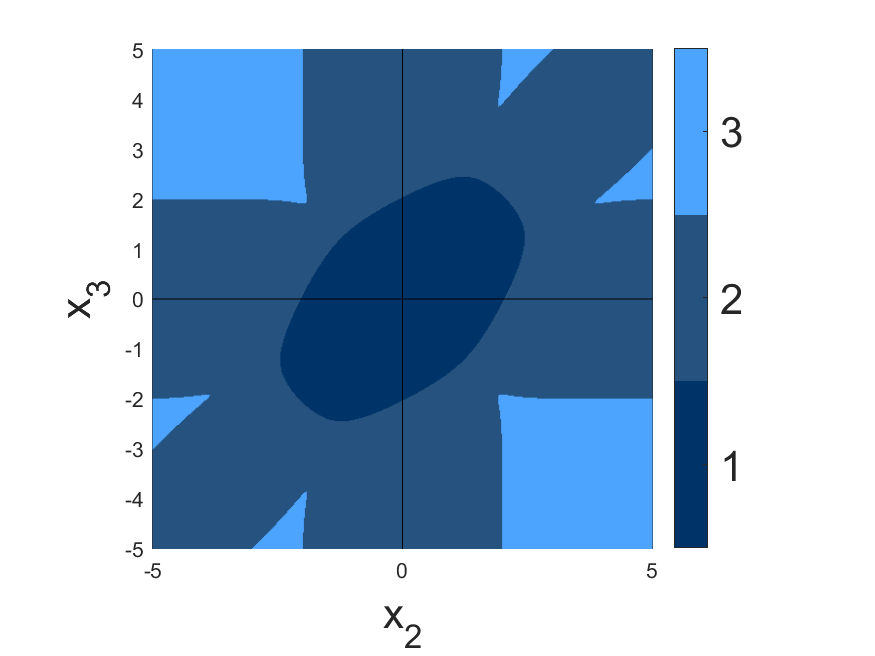
\includegraphics[width=0.9\textwidth]{normal_flag_graph.png}
		\caption{$K_\vect{x}$ as a function of $\vect{x} = (0, x_2, x_3)$ for a normal component density with fixed variance $\sigma^2 = 1$.}\label{fig:normal_flag_graph}
	\end{figure}

	\begin{figure}
		\centering
		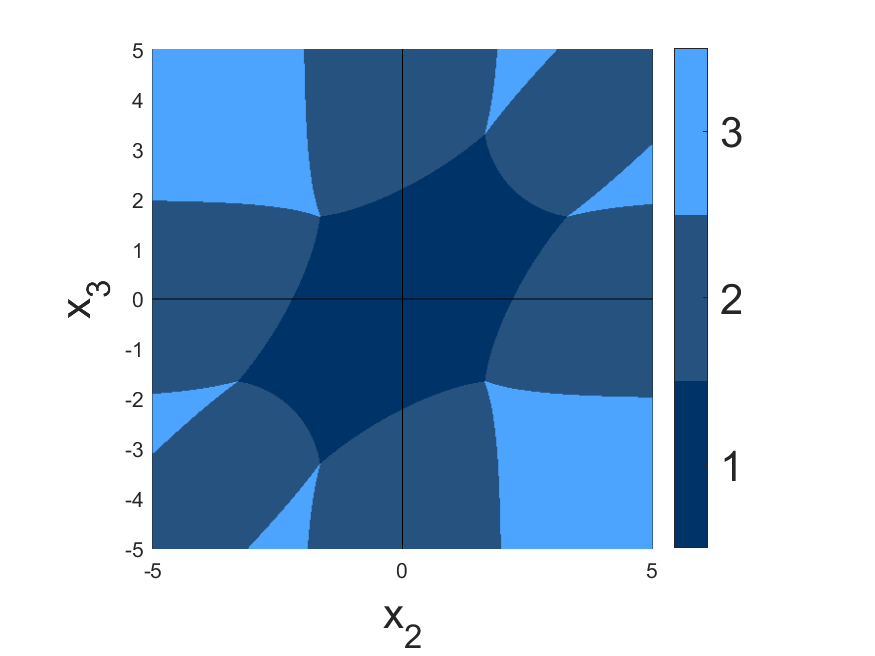
\includegraphics[width=0.9\textwidth]{cauchy_flag_graph.png}
		\caption{$K_\vect{x}$ as a function of $\vect{x} = (0, x_2, x_3)$ for a Cauchy component density with fixed scale $\gamma = \sqrt{3}$.}
		\label{fig:cauchy_flag_graph}
	\end{figure}
	
	While $n = 2,3$ is not a very realistic scenario when it comes to real data to which we may wish to fit a mixture model, it does help demonstrate a particular way of thinking about the problem of determining $K_\vect{x}$. That is, that $K_\vect{x}$ is simply a function of where $\vect{x}$ lies in $\mathbb{R}^n$. For a particular choice of component density, we can partition $\mathbb{R}^n$ into sets 
	\begin{equation}
		C_k = \{ \vect{x} \in \mathbb{R}^n | K_{\vect{x}} = k \}, \hspace{40pt} k = 1,\dots,n.
	\end{equation}
	The problem of determining $K_{\vect{x}}$ is then the same as determining in which of the $C_k$ $\vect{x}$ lies. If $\vect{x} = \vect{X}$ is randomly chosen, then the probability that $K_\vect{X} = k$ is simply the probability that $\vect{X} \in C_k$. In Section \ref{sec:mixture results}, we present various results which bound the regions $C_k$ in various settings.

	[UP TO HERE]

	\section{Results}
	\label{sec:mixture results}

	\subsection{Results for \texorpdfstring{$n = 2$}{n = 2}}
	In this section, we present Theorem \ref{thm:n=2 inflection result} which 
	expands upon the results found in \cite{Lindsay1983-tf} and \cite{Lindsay1983a-he}.

	\subsection{Things that are referenced}
	REWORK CONTENTS OF THIS SUBSECTION INTO MAIN TEXT.
	\begin{equation}
		M(\vect{u}) = \sum_{i=1}^n \log(u_i)
		\label{eq:transformedlikelihood}
	\end{equation}

	\begin{theorem}
		If $\Gamma$ is compact then there exists a unique point on the boundary of $\conv(\Gamma)$ which maximizes the likelihood. This point corresponds to a distribution $Q$ which maximizes the likelihood and that has no more than $n$ point masses.
		\label{thm:LindsayGamma}
	\end{theorem}

	

	\subsection{The likelihood curve for \texorpdfstring{$n = 2$}{n = 2}}
		The shape of $\Gamma_\vect{x}$ can provide us with some insight into the behaviour of $K_\vect{x}$. In Figure \ref{fig:Gammaexample}, we give some examples of $\Gamma_\vect{x}$ for $n=2$ using a normal component density with variance $\sigma^2 = 1$. 
		\begin{figure}[ht]
			\begin{subfigure}[t]{0.32\textwidth}
				\centering
				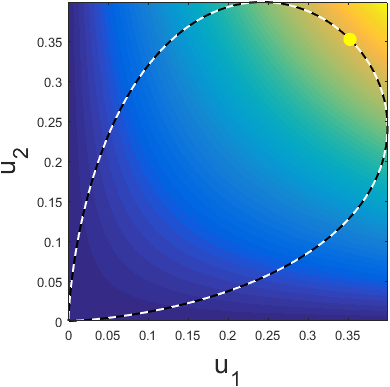
\includegraphics[width = \textwidth]{Sigma1x1_0-x2_1}
				\caption{$\vect{x} = (0,1)$} \label{subfig:gammaexamplea}
			\end{subfigure}
			\begin{subfigure}[t]{0.32\textwidth}
				\centering
				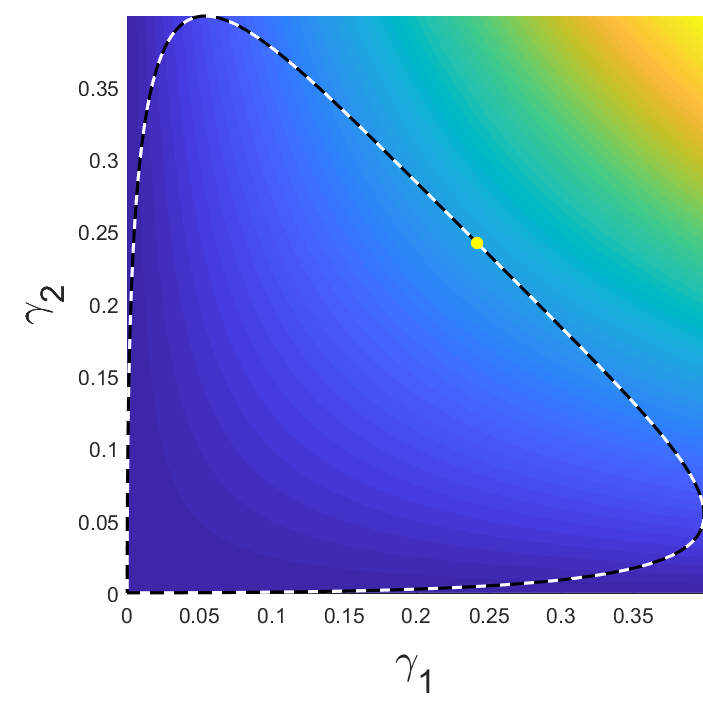
\includegraphics[width = \textwidth]{Sigma1x1_0-x2_2}
				\caption{$\vect{x} = (0,2)$} \label{subfig:gammaexampleb}
			\end{subfigure}
			\begin{subfigure}[t]{0.32\textwidth}
				\centering
				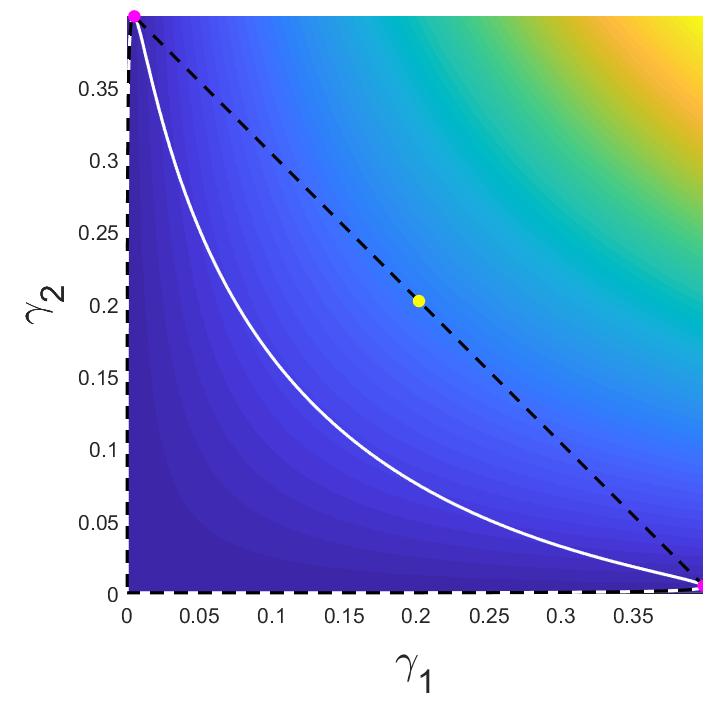
\includegraphics[width = \textwidth]{Sigma1x1_0-x2_3}
				\caption{$\vect{x} = (0,3)$} \label{subfig:gammaexamplec}
			\end{subfigure}
			\caption{The curve $\Gamma_\vect{x}$ for three different $\vect{x}$ along with the boundary of $\conv(\Gamma_\vect{x})$. The objective function, $\mathcal{L}(\vect{\gamma})$, is represented as a heat map. The optimal point $\hat{\vect{\gamma}}$ is shown in yellow, and where applicable, the points $\vect{\gamma}(\theta_j)$ that make up $\hat{\vect{\gamma}}$ are shown in magenta.}
			\label{fig:Gammaexample}
		\end{figure}
		In particular, we note that the distance between $x_1$ and $x_2$ has a strong effect on the shape of $\Gamma_\vect{x}$. In Figure \ref{subfig:gammaexamplea}, the points are distance 1 apart and $\Gamma_\vect{x}$ is the boundary of $\conv(\Gamma_\vect{x})$. In this case, it is clear that $K_\vect{x} = 1$. In Figure \ref{subfig:gammaexamplec}, the points are distance 3 apart and the optimal point no longer lies on $\Gamma_\vect{x}$. This results in the maximum likelihood mixing distribution needing two points of support and so $K_\vect{x} = 2$. The boundary case, where $\Gamma_\vect{x}$ goes from being a convex curve to having the indentation shown in Figure \ref{subfig:gammaexamplec}, is shown in Figure \ref{subfig:gammaexampleb}.

		Obtaining results about where these boundaries lie is very difficult in higher dimensions. In \cite{Lindsay1983a-he}, Lindsay used the sign of the curvature of $\vect{\gamma}(\theta;\vect{x})$ to obtain results for $n=2$ when the component density is in the exponential family. Here we will present an extension to Lindsay's results by considering densities that satisfy the following assumptions.
	
		\begin{assumption}[Continuity]
			$f(x)$ is a continuous density and has the whole real line as its support.
			\label{assump:reallinesupport}
		\end{assumption}
		
		\begin{assumption}[Differentiability]
			$f(x)$ is twice differentiable.
			\label{assump:twicediff}
		\end{assumption}
		
		\begin{assumption}[Unimodality]
			$f(x)$ has a single mode at $x=0$. I.e. $f'(x) > 0$ for $x <0$, $f'(0) = 0$, and $f'(x) < 0$ for $x>0$.
			\label{assump:singlemode}
		\end{assumption}
		
		\begin{assumption}[Symmetry]
			The density $f(x)$ is symmetric about $x = 0$.
			\label{assump:symmetric}
		\end{assumption}
		
		\begin{assumption}
			$f$ has only two points of inflection
			\label{assump:twoinflectionpoints}
		\end{assumption}
		
		\begin{definition}
			If $f$ satisfies assumptions \ref{assump:reallinesupport} through to \ref{assump:singlemode}, then define $[i^-,i^+]$ to be the largest interval that contains 0 and on which $f''(x) \leq 0$.
			\label{def:i-i+}
		\end{definition}
		That is, $i^-$ and $i^+$ are inflection points of $f$. Note that for any $f$ satisfying \ref{assump:symmetric}, $i^- = -i^+$. In this case we will write $i = i^+ = -i^-$.
		
		\begin{assumption}
			$f'(x) > -f'(x - 2i)$ for $\theta \in (i,\infty)$
			\label{assump:magnitudegradients}
		\end{assumption}
		
		Some common densities that satisfy these assumptions include the normal density and the Cauchy density.
		
		\begin{lemma}
			\label{lem:magnitudegradients}
			% Prove stuff about magnitude of gradients (i.e. $\gamma_x < \gamma_y$)
			Let $f(x)$ be a density which satisfies assumptions \ref{assump:reallinesupport} through to \ref{assump:magnitudegradients} and whose inflection points are at $x=i$ and $x=-i$. If 
			$x_2 - x_1 < 2i$ ($x_2 > x_1$) then the equation
			\begin{equation}
				-f'(x_1 - \theta) = f'(x_2 - \theta)
				\label{eq:gradientsequal}
			\end{equation}
			has only one solution.
		\end{lemma}
		\begin{proof}
			We first consider the shape of $f'(x)$. Assumption \ref{assump:singlemode} tells us that $f'(x)$ is positive for $x<0$ and negative for $x>0$. The function $f'(x)$ will have turning points at $\pm i$ and from Assumption \ref{assump:twoinflectionpoints} these will be the only turning points. Hence we have the following picture of $f'(x)$:
			\begin{equation}
				f'(x) \text{ is } 
				\begin{cases}
					\text{positive and increasing,} &x \in (-\infty,-i)\\
					\text{positive and decreasing,} &x \in (-i,0)\\
					\text{negative and decreasing,} &x \in (0,i)\\
					\text{negative and increasing,} &x \in (i,\infty).
				\end{cases}
			\end{equation}
			We also note, from \ref{assump:symmetric}, that $f'(x)$ is an odd function. Using this and rearranging \eqref{eq:gradientsequal} we obtain the equivalent equation
			\begin{equation}
				g(\theta) = h(\theta)
				\label{eq:gradientsequalequivalent}
			\end{equation}
			where we have put $g(\theta) = f'(\theta)$ and $h(\theta) = -f'(\theta - (x_2 - x_1))$ for ease of notation.
			% We now make the assumption that $0<x_2 - x_1<2i$
			% Since $x_2 > x_1$, the right hand side of \eqref{eq:gradientsequalequivalent} is $-f'(x)$ translated to the right by $x_2 - x_1$. Since $x_2 - x_1 < 2i$, the positive turning point of $-f'(\theta - (x_2 - x_1))$ satisfies
			% \begin{equation}
			% -i + x_2 - x_1 < i,
			% \end{equation}
			% that is, it comes before the positive turning point of $f'(\theta)$.
			
			If we assume that $0< x_2 - x_1 < 2i$ then we can consider possible solutions to \eqref{eq:gradientsequalequivalent} on each of the following intervals. 
			
			For $\theta \in (-\infty, 0]$, $g(\theta)\geq 0$ and $h(\theta) < 0$ and so there are no possible solutions.
			
			Likewise, for $\theta \in [x_2 - x_1,\infty)$, $g(\theta)<0$ and $h(\theta) \geq 0$ and so there are no possible solutions.
			
			For $\theta \in [-i + x_2 - x_1,i]$, $g(\theta)$ is decreasing and $h(\theta)$ is increasing and $h(-i+x_2 -x_1) = g(i)$ (since $f'$ is odd). Therefore there must be exactly one solution in this interval.
			
			We note that if $x_2 - x_1 \leq i$ then the above intervals cover the real line. In the case that $i <x_2 - x_1 < 2i$ we need to consider these additional intervals.

			For $\theta \in (i,x_2 - x_1)$, from assumption \ref{assump:magnitudegradients}, $f'(\theta) < -f'(\theta - 2i) < -f'(\theta - (x_2 - x_1))$ since both $-f'(\theta - 2i)$ and $-f'(\theta - (x_2 - x_1))$ are increasing on this interval. Hence there can be no solutions to \eqref{eq:gradientsequalequivalent} on this interval.
			
			Similarly by symmetry of $f$, for $\theta \in (0,-i+x_2-x_1)$,  $f'(\theta)>-f'(\theta - 2i) > -f'(\theta - x_2 - x_1)$ and there are no solutions to \eqref{eq:gradientsequalequivalent} on this interval either.
			
			Since the above intervals cover the real line and since we have shown that there is only one solution in one of these intervals, \eqref{eq:gradientsequal} must have only one solution.
		\end{proof}
		
		\begin{theorem}
			\label{thm:n=2 inflection result}
			Let $f(x)$ satisfy assumptions \ref{assump:reallinesupport} through to \ref{assump:magnitudegradients}. Let $\vect{x} = (x_1,x_2)$ be the sample for which we a finding a maximum likelihood mixture using $f$ as the component density. Then $K_\vect{x} = 1$ if and only if
			\begin{equation}
				x_2 - x_1 \leq 2i
				\label{eq:x2-x1<int}
			\end{equation}
		\end{theorem}
		\begin{proof}
			% Since $f(x)$ has a single mode at $x = 0$, the points of support of the maximizing mixing distribution must lie between $x_{1}$ and $x_{2}$. Hence we are
			By the unimodality of $f$, the points of support of the maximizing mixing distribution must lie between $x_1$ and $x_2$. Hence we need only consider the behaviour of $\vect{\gamma}(\theta;\vect{x})$ for $\theta \in [x_1,x_2]$. By the symmetry of $f$, $\hat{\vect{u}}$ must lie on the line $u_1 = u_2$\footnote{This is obvious but may need a lemma}.
			
			First we complete the only if direction of the proof. Assume that $x_2 - x_1 > 2i$. By the symmetry of $f$, $\vect{\gamma}(\theta;\vect{x})$ crosses the $u_1 = u_2$ line at $\theta = (x_1 + x_2)/2$. Now the curvature of $\vect{\gamma}$ has sign equal to
			
			\begin{equation}
				S(\theta) = 
				\begin{vmatrix}
					\gamma_1'(\theta;\vect{x})&\gamma_1''(\theta;\vect{x})\\
					\gamma_2'(\theta;\vect{x})&\gamma_2''(\theta;\vect{x})
				\end{vmatrix} = 
				\begin{vmatrix}
					-f'(x_1 - \theta) & f''(x_1 - \theta)\\
					-f'(x_2 - \theta) & f''(x_2 - \theta)
				\end{vmatrix}.
			\end{equation}
			and so
			\begin{equation}
				S\left(\frac{x_1+x_2}{2}\right) = 
				\begin{vmatrix}
					-f'(\frac{x_1 - x_2}{2}) & f''(\frac{x_1 - x_2}{2})\\
					-f'(\frac{x_2 - x_1}{2}) & f''(\frac{x_2 - x_1}{2})
				\end{vmatrix}.
			\end{equation}
			Since $x_2 - x_1 > 2i$, $\frac{x_1 - x_2}{2} > i$ and so $f''((x_1 - x_2)/2) > 0$. Similarly, $f''((x_2 - x_1)/2)>0$. We also have that $-f((x_1 - x_2)/2) < 0$ and $-f((x_2 - x_1)/2) > 0$. Hence $S((x_1 + x_2)/2)<0$ and so $\vect{\gamma}((x_1 + x_2)/2;\vect{x})$ has negative curvature. The curve $\Gamma$ must have positive curvature at the points of support and so we cannot have that $K_\vect{x} = 1$.
			
			Now we complete the if direction. Assume that $x_2 - x_1 \leq 2i$. By Lemma \ref{lem:magnitudegradients}, there is only one point at which the curve is pointing perpendicular to the line $u_1 = u_2$ SAY THIS BETTER. By the symmetry of $f$ this occurs when $\gamma(\theta;\vect{x})$ is crossing the line $u_1 = u_2$. Since $f$ is continuous, the direction that $\gamma(\theta;\vect{x})$ is moving is also continuous. At $\theta = x_1$, $\gamma(\theta;\vect{x})$ is pointing straight up and so we have that for $\theta \in [x_1,(x_1 + x_2)/2]$, $\gamma(\theta;\vect{x})$ is travelling in a direction pointing above the line perpendicular to $u_1 = u_2$. For $\theta \in [(x_1 + x_2)/2,x_2]$, $\gamma(\theta;\vect{x})$ points below the line. It is now obvious that $\gamma((x_1 + x_2)/2;\vect{x})$ is the furthest point from the origin that lies on $u_1 = u_2$ and is in the convex hull of $\Gamma_\vect{x}$. Since the likelihood increases as we move away from the origin along the line $u_1 = u_2$ in the positive quadrant, we must have
			$$\hat{\vect{u}} = \gamma((x_1 + x_2)/2;\vect{x})$$
			and so $K_\vect{x} = 1$.
			
			% Basic idea just here - 		
			% Now either made up of two points or lies on $\Gamma_\vect{x}$. If made up of two points then these two points are symmetrical about $u_1 = u_2$ and the part of $\Gamma_\vect{x}$ that crosses $u_1 = u_2$ is closer to origin. However, if angle of $\gamma$ is always above angle that is perpendicular to $u_1 = u_2$ before crossing $u_1 = u_2$ then impossible for point where it crosses to be closer to origin than that of line between any two symmetrical points.
		\end{proof}

\section{Results for general n}
	
	\subsection{Normal Constraints}
		When our component density is normal with variance $\sigma^2$,
		\begin{equation}
			f(x;\sigma) = \frac{1}{\sigma \sqrt{2\pi}} \euler^{-x^2/2\sigma^2},
		\end{equation}
		equations \eqref{eq:Deq1} to \eqref{eq:Deq3} become
		\begin{align}
			&\frac{1}{n} \sum_{i=1}^n \Gamma_k(x_i;\vect{p},\vect{\theta}) = 1 \label{eq:GammaEq1}\\
			&\frac{1}{n} \sum_{i=1}^n x_i \Gamma_k(x_i;\vect{p},\vect{\theta}) = \theta_k \label{eq:GammaEq2}\\
			&\frac{1}{n} \sum_{i=1}^n (x_i - \theta_k)^2 \Gamma_k(x_i;\vect{p},\vect{\theta}) \leq \sigma^2
			\label{eq:GammaEq3}
		\end{align}
		where we have written
		\begin{equation}
			\Gamma_k(x;\vect{p},\vect{\theta}) = \frac{f(x - \theta_k;\sigma)}{\sum_{j=1}^m p_j f(x - \theta_j;\sigma)}.
		\end{equation}
		for ease of notation. Using these constraints, we will bound the regions
		$C_1, \dots, C_n$ in Theorem \ref{thm:general n constraints result}. However, as a gentle introduction we will start with the much simpler problem of just bounding $C_1$.

		\begin{theorem}
			\label{thm:general n C1 bound}
			Write $\bar{\vect{x}}$ for the mean of $\vect{x}$. If $\vect{x} \in C_1$ then 
			\begin{equation}
				\frac{1}{n} \sum_{i=1}^n (x_i - \bar{\vect{x}})^2 \leq \sigma^2.
			\end{equation}
		\end{theorem}
		\begin{proof}
			If $\vect{x} \in C_1$ then the maximizing mixture has one component and so $\Gamma_1(x; \vect{\theta}, \vect{p}) = 1$. Then \eqref{eq:GammaEq2} gives us that $\theta_1 = \bar{\vect{x}}$ and combining this with \eqref{eq:GammaEq3} completes the proof.
		\end{proof}

	\subsubsection{Treating \texorpdfstring{$\vect{x}$}{x} as random}

		Up until now, we have treated $\vect{x}$ as fixed, not random, and treated the maximum likelihood problem purely as an optimization one, rather than a statistical one. However, for this section we make the assumption that $\vect{x}$ is made up of i.i.d. random variables, $x_i$, which have distribution
		$$x_i \sim N(\mu,\sigma_1^2)$$
		for $i = 1,\dots,n$. Our component density, $f_\theta$, is normal with variance $\sigma_2^2$. From Theorem \ref{thm:general n C1 bound},
		\begin{align*}
		p_u &= \prob \left( \sum_{i=1}^n (x_i - \bar{\vect{x}})^2 \leq n \sigma_2^2  \right)
		\end{align*}
		is an upper bound to $\prob(\vect{x} \in C_1)$. Writing $s^2$ for the unbiased sample variance of $\vect{x}$
		\begin{align*}
		p_u 
		%&= \prob\left( \frac{1}{n-1} \sum_{i=1}^n (x_i - \bar{x})^2 \leq \frac{n\sigma}{n-1}\right)\\
		&= \prob\left( s^2 \leq \frac{n \sigma_2^2}{n-1}\right)\\
		&= \prob\left( \frac{(n-1)s^2}{\sigma_1^2} \leq \frac{n \sigma_2^2}{\sigma_1^2}\right)\\
		&= \prob\left(\chi_{n-1}^2  \leq \frac{n \sigma_2^2}{\sigma_1^2} \right)
		\end{align*}
		where $\chi_{n-1}^2$ is chi-squared with $n-1$ degrees of freedom.

		\begin{remark}
			Of particular interest is the case where $\sigma_1 = \sigma_2$. In this case, $p_u \rightarrow 1/2$ as $n \rightarrow \infty$. While not a new result [CITE SOMETHING HERE], this tells us that the maximum likelihood estimator is not a consistent estimator for the number of components.
		\end{remark}

		% From Theorem \ref{thm:shapeofC1normalb}, an lower bound to $\prob(\vect{x} \in C_1)$ is
		% \begin{align*}
		% p_l &= \prob(x_{(n)} - x_{(1)} < 2\sigma)\\
		% 	&\geq \prob(\mu - \sigma < x_{(1)} < x_{(n)} < \mu + \sigma )\\
		% 	&=  \left(\int_{\mu - \sigma}^{\mu + \sigma} f(x) \intd x \right)^n\\
		% 	&= \left( \erf\left(\frac{\sigma_2}{\sqrt{2}\sigma_1}\right)\right)^n
		% \end{align*}

	\subsection{Properties of \texorpdfstring{$\Gamma$}{Gamma}}
		In order to bound regions where $m \geq 2$, we will need to get a handle on $\Gamma_k(x;\vect{\theta}, \vect{p})$. In this section, we list and prove some properties that will be required in Section \ref{sec:bounding Cm}.

		\begin{lemma}
		\label{lem:maxkGamma}
			\begin{equation}
				\max_k \left( \Gamma_k(x;\vect{p},\vect{\theta}) \right) \geq 1
			\end{equation}
		\end{lemma}	
		\begin{proof}
			For each $x$, there exists a $k_0$ such that $f(x - \theta_{k_0};\sigma) \geq f(x - \theta_k;\sigma)$ for all $k$. It follows that
			\begin{equation}
				\Gamma_{k_0}(x;\vect{p},\vect{\theta}) = \frac{f(x - \theta_{k_0};\sigma)}{\sum_{j=1}^m p_j f(x - \theta_j;\sigma)} \geq \frac{f(x - k_0;\sigma)}{\sum_{j=1}^m p_j f(x - \theta_{k_0};\sigma)} = 1.
			\end{equation}
		\end{proof}

		\begin{lemma}
			\begin{equation}
			\Gamma_k(x;\vect{p},\vect{\theta}) \leq \frac{1}{p_k}
			\end{equation}
		\end{lemma}
		\begin{proof}
			Since $f(x) > 0$,
			\begin{equation}
				\Gamma_k(x;\vect{p},\vect{\theta}) = \frac{f(x - \theta_k;\sigma)}{\sum_{j=1}^m p_j f(x - \theta_j;\sigma)} \leq \frac{f(x - \theta_k;\sigma)}{p_k f(x - \theta_k;\sigma)} = \frac{1}{p_k}.
			\end{equation}
		\end{proof}

		\begin{lemma}
			Let $\gamma(x)$ be a non-negative function that satisfies
			\begin{equation}
				\frac{1}{n} \sum_{i=1}^n \gamma(x_i) = 1.
			\end{equation}

			Then the $\theta$ that minimizes 
			\begin{equation}
				\frac{1}{n} \sum_{i=1}^n (x_i - \theta)^2 \gamma(x_i)
			\end{equation}
			is
			\begin{equation}
				\theta = \frac{1}{n} \sum_{i=1}^n x_i \gamma(x_i).
			\end{equation}
		\end{lemma}
		\begin{proof}
			CURRENTLY UNUSED. PROOF IN TIM'S NOTEBOOK.
		\end{proof}

	\subsection{Bounding \texorpdfstring{$C_m$}{Cm}}
	\label{sec:bounding Cm}
		\begin{theorem}
			THM AND PROOF IS BELOW
			\label{thm:general n constraints result}
		\end{theorem}
		Let $\vect{x} = (x_1,\dots,x_n)$ and assume that the maximum likelihood mixture for $\vect{x}$ has no more than $m$ components. Let $\hat{\vect{\theta}}$ and $\hat{\vect{p}}$ denote this maximizing mixture. %Let $\hat{\vect{\theta}} = (\hat{\theta}_1,\dots,\hat{\theta}_m)$ and $\hat{\vect{p}} = (\hat{p}_1,\dots,\hat{p}_m)$ be a maximizing mixture for $\vect{x}$
		Then by Lemma \ref{lem:maxkGamma}, there exists a $k^*$ such that $\Gamma_{k^*}(x_i;\hat{\vect{p}},\hat{\vect{\theta}}) \geq 1$ for at least $\lceil \frac{n}{m} \rceil$ different $x_i$. Let $A_{k^*}$ be the set of all these $x_i$. 
		Let $A_{\theta_{k^*}}$ be the set of the $|A_{k^*}|$ closest $x_i$ to $\theta_{k^*}$. Then
		\begin{align}
			\frac{1}{n} \sum_{i=1}^n (x_i - \theta_{k^*})^2 \Gamma_{k^*}(x_i; \hat{\vect{p}},\hat{\vect{\theta}}) &\geq \frac{1}{n} \sum_{i \in A_{\theta_{k^*}}} (x_i - \theta_{k^*})^2 \\
			&\geq \frac{1}{n} \left \lceil \frac{n}{m} \right \rceil \var\left(A_{\theta_{k^*}}\right) &&\text{(Biased Variance)}
		\end{align}

		From \eqref{eq:GammaEq3},
		\begin{equation}
			\var\left(A_{\theta_{k^*}}\right) \leq \frac{n \sigma^2}{\left\lceil \frac{n}{m} \right\rceil}.
		\end{equation}

		This means that if we cannot find a subset of the $x_i$ that has at least $\frac{n}{m}$ elements and has (biased) variance less than $\frac{n\sigma^2}{\left\lceil \frac{n}{m} \right\rceil}$ then we need more than $m$ components in our maximum likelihood mixture.


	\subsection{A particular class of optimization problem}
		"The results follow from this general theorem which seems obvious."

		\begin{theorem}
			\label{thm:solution in interior}
			Let $(E_m)_{m=1}^\infty$ be a sequence of appropriately defined sets and let
			$(g_m)_{m=1}^\infty, g_m: E_m \mapsto \mathbb{R}$ be a sequence of
			functions that satisfy the following properties
			\begin{enumerate}
				\item $\forall \vect{x} \in \partial E_m, \exists n < m, \vect{y} \in E_n$ such that
				$g_m(\vect{x}) \leq g_n(\vect{y})$.
				\label{prop:one}
				\item $\exists m_0, \vect{x}_0 \in E_{m_0}$ such that $\forall m, \vect{x} \in 
				E_m$, $g_m(\vect{x}) \leq g_{m_0}(\vect{x}_0)$.
			\end{enumerate}
			Then $\exists m_*, \vect{x}_* \in E_{m_*} \setminus \partial E_{m_*}$ such
			that $\forall m, \vect{x} \in E_m$, $g_m(\vect{x}) \leq g_{m_*}(\vect{x}_*)$.
		\end{theorem}
		\begin{proof}
			The proof is simple. If $\vect{x}_0 \notin \partial E_{m_0}$ then we are done.
			Otherwise, by property \ref{prop:one} we can find a $n$ and $\vect{y} \in 
			E_n$ such that $g_n(y) = g_{m_0}(\vect{x}_0)$. If $\vect{y} \notin \partial 
			E_n$ then we are done, otherwise we repeat the process until we find a $m, 
			\vect{x}$ pair with $\vect{x} \notin \partial E_m$. %Note that property 
			% \ref{prop:one} implies that $\partial E_1 = \emptyset$ and so this process
			% must end.
		\end{proof}

	\subsection{Derive Constraints again}
	WE SHOULD BE ABLE TO DERIVE \eqref{eq:GammaEq1} THROUGH \eqref{eq:GammaEq3} AGAIN USING THEOREM \ref{thm:solution in interior}.

% \section{Other Results}
	\subsection{All points separated by \texorpdfstring{$\alpha$}{a}}
		Consider the situation in which $|x_i - x_j| > \alpha$ for all $i\neq j$. Intuitively, we would expect that there is some $\alpha^*$ such that if $\alpha > \alpha^*$ then $\vect{x} \in C_n$.
		
		\begin{theorem}
			If our component density is unimodal and symmetric about zero, and
			$$\frac{f(\alpha/2)}{f(0)} < \frac{1}{n}\left(\frac{n-1}{n}\right)^{n-1}.$$
			Then if $|x_i - x_j| > \alpha$ for all $i\neq j$, $\vect{x} \in C_n$.
		\end{theorem}
		\begin{proof}
			Let $\hat{f}_{n-1}$ be the maximum likelihood mixture density of $\vect{x}$ with no more than $n-1$ components and let $L_{n-1}$ be the corresponding likelihood. Since all the $x_i$ are separated by at least $\alpha$, there exists an $x_{i^*}$ such that $|x_{i^*} - \theta_j|>\frac{\alpha}{2}$ for all $j$. Hence
			$$\hat{f}_{n-1}(x_{i^*}) < f(\alpha/2)$$
			and so
			$$L_{n-1} < f(\alpha/2) \prod_{i\neq i^*} \hat{f}_{n-1}(x_{i}).$$
			
			We will now construct a mixture density that has one more component that $\hat{f}_{n-1}$. We do this by scaling all the components of $\hat{f}_{n-1}$ by a factor of $\frac{n-1}{n}$ and introducing a new component with parameters $(p,\theta) = (\frac{1}{n},x_{i^*})$. Call this function $f^*_n$ and the corresponding likelihood $L_n$. Now
			
			$$L_n > \frac{f(0)}{n} \left(\frac{n-1}{n}\right)^{n-1}\prod_{i\neq i^*} \hat{f}_{n-1}(x_i).$$
			
			So if $f(\alpha/2) < \frac{f(0)}{n} \left(\frac{n-1}{n}\right)^{n-1}$ then $L_n > L_{n-1}$ and so $\vect{x} \in C_n$.
		\end{proof}

	\subsection{Discussion about what we hope to acheive}
		The few original results above (Theorems \ref{thm:n=2 inflection result} and \ref{thm:general n constraints result}) seem to be special cases of what looks to be a much more general rule. Theorem \ref{thm:general n constraints result} seems to be too large by a factor of $m$ when you compare to numerics, and the distance between inflection points in Theorem \ref{thm:n=2 inflection result} seems to come up again when when you look at images like Figure \ref{fig:normal_flag_graph} (eg the thickness of the `bands' is this distance). It is therefore our hope that we can either generalize or add significantly to the Theorems stated so far.